%%%%%%%%%%%%%%%%%%%%%%%%%%%%%%%%%%%%%%%%%%%%%%%%%%
%%%%%%%%%%%%%%%%%%%%%%%%%%%%%%%%%%%%%%%%%%%%%%%%%%
% INTRODUÇÃO
%%%%%%%%%%%%%%%%%%%%%%%%%%%%%%%%%%%%%%%%%%%%%%%%%%
%%%%%%%%%%%%%%%%%%%%%%%%%%%%%%%%%%%%%%%%%%%%%%%%%%

\section{Introdução}
Este documento está associado ao primeiro exercício prático da matéria de Teoria dos Grafos e Computabilidade (TGC). Esse exercício exigiu a solução de problemas recorrentes no mundo de grafos, nos pedindo para implementar algoritmos reconhecidos, como Naive, Tarjan, Fleury e Brute Force. Esses algoritmos são utilizados para identificar a conectividade nos grafos, identificar componentes fortemente conexos, identificar caminhos eulerianos e identificar pontes, respectivamente.


%%%%%%%%%%%%%%%%%%%%%%%%%%%%%%%%%%%%%%%%%%%%%%%%%%
%%%%%%%%%%%%%%%%%%%%%%%%%%%%%%%%%%%%%%%%%%%%%%%%%%
% TRABALHOS RELACIONADOS
%%%%%%%%%%%%%%%%%%%%%%%%%%%%%%%%%%%%%%%%%%%%%%%%%%
%%%%%%%%%%%%%%%%%%%%%%%%%%%%%%%%%%%%%%%%%%%%%%%%%%

\subsection{Motivação}
Colocar em prática a teoria aprendida em sala de aula, gerando mais familiaridade e entendimento sobre o assunto, incentivando um maior estudo prático da matéria a partir da implementação dos diferentes códigos abordados em sala de aula.
\subsection{Objetivos}
Identificar pontes através dos algoritmos de Tarjan e Naive, e através do uso desses dois algoritmos, somos capazes de executar o algoritmo de Fleury para identificar os caminhos eulerianos no grafo.
\subsection{Grafo Utilizado}
Utilizamos o grafo ilustrado na figura \ref{fig:grafo} para a realização dos nossos testes em código. Grafo conexo, não direcionado com 5 vértices e 5 vértices, o suficiente para testar tudo o que foi solicitado no trabalho.
\begin{figure}[H]
	\centering	
    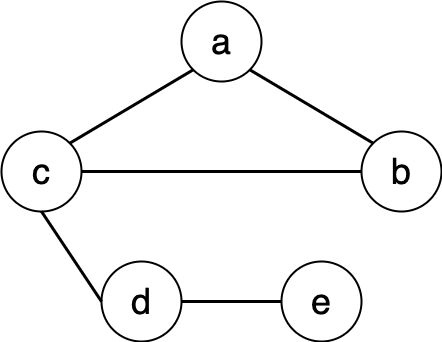
\includegraphics[width=.50\linewidth]{Figuras/Graph.png}
    \caption{Grafo utilizado para os testes no código.}
    \label{fig:grafo}
\end{figure}



%%%%%%%%%%%%%%%%%%%%%%%%%%%%%%%%%%%%%%%%%%%%%%%%%%
%%%%%%%%%%%%%%%%%%%%%%%%%%%%%%%%%%%%%%%%%%%%%%%%%%
% Algoritmos
%%%%%%%%%%%%%%%%%%%%%%%%%%%%%%%%%%%%%%%%%%%%%%%%%%
%%%%%%%%%%%%%%%%%%%%%%%%%%%%%%%%%%%%%%%%%%%%%%%%%%

\newpage
\section{Algoritmos Implementados}
Nessa seção do texto, aprofundaremos nos algoritmos implementados nesse trabalho.
\subsection{Tarjan}
O algoritmo de \textit{Tarjan} foi implementado primeiramente para a identificação de \textit{Strongly Connected Component} (SCC), em portugês Componentes Fortemente Conexos em grafos direcionados.

O algoritmo de \textit{Tarjan} foi utilizado apenas como uma base para uma adaptação feita na finalidade do algoritmo, que assim como falado acima, foi criado para a identificação de componentes fortemente conexos nos grafos direcionados, mas como estamos trabalhando com grafos não-direcionados, não faz sentido buscarmos essas compontentes, tendo em vista que elas não existem para esse tipo de grafo. O algoritmo de \textit{Tarjan} implementado no presente trabalho tem como objetivo identificar possíveis pontes no grafo. Para essa implementação, seguimos a ideia do \textit{Tarjan} utilizando os \textit{ID's} e \textit{Low Link Values} para cada vértice do grafo, e através de uma \textit{Deep First Search} (DFS), também conhecida como Busca em Profundidade a fim de modificarmos os valores nas listas de \textit{ID's} e \textit{Low Link Values} de cada vértice. Após definirmos os valores nas listas, fazemos as devidas verificações para identificarmos as arestas de ponte. Caso o \textit{Low Link Values} do atual for maior que o \textit{ID} do vértice sucessor, significa que estão em componentes distintos, logo caso a aresta que liga os dois vértices for removida do grafo, teremos dois componentes, logo a aresta é uma ponte.

\subsubsection{Pseudocódigo}
% algoritmo
% \begin{figure}[ht]
\begin{center}	
	\vspace{-0.3cm}
\begin{minipage}[ht]{13cm}
\begin{algorithm}[H]
  \footnotesize
  \caption{Algoritmo Tarjan}
  \label{alg:2}
  \begin{algorithmic}[2]
     \STATE \textbf{Entrada:} vértice Atual e vértice Anterior
     \STATE \textbf{Saída:} Uma lista contendo os vértices de ponte encontrados.
     \STATE G = \textbf{GRAFO}
     \STATE stack.$push$($atual$)
     \STATE onStack[$atual$] = $true$
     \STATE ids[$atual$] = low[$atual$] = id++
     
    \FOR{$sucessor$ in $sucessores$[$atual$]}
        \IF{ids[$sucessor$] == -1}
            \STATE TARJAN($sucessor$, $atual$)
        \ENDIF
        \IF{$sucessor$ != $anterior$ && onStack[$sucessor$] == \texbf{TRUE}}
            \STATE low[$atual$] = min(low[$atual$], low($sucessor$))
        \ENDIF
        \IF{low[$sucessor$] > ids[$atual$]}
            \STATE resposta.$append$($concat$($atual$, $sucessor$))
        \ENDIF
    \ENDFOR
    \IF{ids[$atual$] == low[$atual$]}
        \FOR{$vert$ in $stack$}
            \STATE onStack[$vert$] = false
            \STATE stack.$pop$()
            \STATE low[$vert$] = ids[$vert$]
            \IF{$vert$ == $atual$}
                \STATE \texbf{BREAK}
            \ENDIF
        \ENDFOR
    \ENDIF
    \STATE \textbf{Retorna} resposta; FIM
  \end{algorithmic}
\end{algorithm}
\caption{Algoritmo 2 - Naive}
\end{minipage}
\end{center}

\subsection{Naive}

O algoritmo \textit{Naive} foi implementado para identificar, de maneira direta, arestas que são pontes em um Grafo.

O algoritmo \textit{Naive}, também chamado de \textit{Brute Force}, Força bruta em português, tem como ideia principal analisar um vértice do Grafo por vez, e no final, identificar todos as pontes existentes. Inicialmente é selecioado uma aresta qualquer, remove-se ela do conjunto de arestas, e executa um caminhamento de profundidade no Grafo com o novo conjunto de arestas. Ao final do caminhamento é analisado a quantidade total de vértices visitados no caminhamento, caso o número de vértices visitados seja menor do que a quantidade de vértices no Grafo, podemos afirmar que a aresta analisada é uma ponte.
\subsubsection{Pseudocódigo}


% algoritmo
% \begin{figure}[ht]
\begin{center}	
	\vspace{-0.3cm}
\begin{minipage}[ht]{13cm}
\begin{algorithm}[H]
  \footnotesize
  \caption{Algoritmo Naive}
  \label{alg:2}
  \begin{algorithmic}[2]
     \STATE \textbf{Saída:} Uma lista contendo os vértices de ponte encontrados.
     \STATE G = \textbf{GRAFO}
     \STATE visitado[$aresta$] = \textbf{nova lista}
     \STATE resposta = \textbf{nova lista}
     
    \FOR{$aresta$ in $Arestas$}
        \IF{visitado[$aresta$] == \textbf{false}}
            \STATE visitado[$aresta$] = \textbf{true}
            \STATE G.$removeAresta$($aresta$)
            \STATE resultado = G.$DFS()$
            \IF{resultado.$size$ != G.$vert$.$size()$}
                \STATE resposta.$append(aresta)$
            \ENDIF
            \STATE G.$adicionaAresta$($aresta$)
        \ENDIF
    \ENDFOR
    \STATE \textbf{Retorna} resposta; FIM
  \end{algorithmic}
\end{algorithm}
\caption{Algoritmo 2 - Naive}
\end{minipage}
\end{center}

\subsection{Fleury}
O algoritmo de \textit{Fleury} foi implementado com duas maneiras distintas de identificação de pontes para a definição do vértice inicial do nosso caminho. Primeiramente usamos o algoritmo de \textit{Tarjan} modificado, que foi explicado anteriormente, e no segundo momento utilizamos o algoritmo \textit{Naive} para a identificação dessas pontes.

O algoritmo de \textit{Fleury} tem como papel principal a identificação de caminhos ou ciclos eulerianos em um Grafo, caso existam. A ideia central é identificar a quantidade de vértices com grau ímpar o Grafo possui. Caso seja 0, teremos um ciclo euleriano, e caso seja 2, um caminho euleriano. Com um ciclo euleriano, poderemos começar o caminhamento por qualquer vértice desejado, já no caminho euleriano, teremos que começar por um vértice de grau ímpar.

Após decidirmos qual vértice começar, deve-se identificar as pontes momentâneas, caso o vértice escolhido só tenha sucessores em arestas pontes, caminharemos para um sucessor qualquer, caso tenha arestas não pontes, devemos obrigatoriamente caminhar para ela.

\subsubsection{Pseudocódigo}
 

% algoritmo
% \begin{figure}[ht]
\begin{center}	
	\vspace{-0.3cm}
\begin{minipage}[ht]{13cm}
\begin{algorithm}[H]
  \footnotesize
  \caption{Algoritmo Fleury}
  \label{alg:2}
  \begin{algorithmic}[2]
     \STATE \textbf{Saída:} Uma lista contendo os vértice do caminho ou ciclo euleriano do Grafo.
     \STATE G = \textbf{GRAFO}
     \STATE visitado[$aresta$] = \textbf{nova lista}
     \STATE resposta = \textbf{nova lista}
     \STATE bucket = \textbf{nova pilha}
     \STATE vInicial = \textbf{novo vertice}
     \IF{Numero de vértices com grau ímpar \textit{==} 0}
        \STATE vInicial = vértice qualquer em G
     \ELSE
        \STATE vInicial = vértice de grau ímpar qualquer em G
     \ENDIF
     
     \STATE bucket.$push$($vInicial$)
     \WHILE{!bucket.$empty()$}
        \STATE encontrado = \textit{false}
        \STATE vRemovido = bucket.$pop$()
        \STATE removedSuc = sucessores de vRemovido
        
        \STATE pontes = $ALGORITMO (TARJAN/NAIVE)$
        
        \WHILE{!removedSuc.$empty()$}
            \STATE vVerificado = removedSuc.$pop$()
            \IF{vVerificado não contido em \textbf{pontes}}
                \STATE vCaminhado = vVerificado
                \STATE removedSuc.$clear$()
                \STATE encontrado = \textit{true}
            \ENDIF
        \ENDWHILE
        \IF{encontrado \textit{!=} \textbf{TRUE}}
            \STATE vCaminhado = vVerificado
        \ENDIF
        
        \STATE arestaRemover = $concat$($vRemovido$, $vCaminhado$)
        \STATE G.$removeAresta$($arestaRemover$)
        \STATE bucket.$push$($vCaminhado$)
        \STATE resposta.$push$($vCaminhado$)
        
     \ENDWHILE

    \STATE \textbf{Retorna} resposta; FIM
  \end{algorithmic}
\end{algorithm}
\caption{Algoritmo 3 - Fleury}
\end{minipage}
\end{center}

\newpage
\section{Conclusão}
\label{Conclusao}
Identificar todos as pontes e caminhos Eulerianos em um Grafo é uma tarefa árdua que porém pode ter muitas utilidades na computação. No trabalho em questão utilizamos duas abordagens para identificação de pontes (\textit{Naive} e \textit{Tarjan}) diferentes para verificar se a conectividade no Grafo se altera com a remoção de uma aresta e a outra abordagem utilizada no trabalho foi para a identificação de caminhos ou ciclos Eulerianos com o algoritmo de \textit{Fleury} em duas versões distintas, na primeira, investigamos se uma aresta é ponte ou não através do algoritmo de \textit{Tarjan} e na segunda abordagem, utilizamos o algoritmo de \textit{Naive} para a identificação das mesmas pontes, e os resultados encontrados não foram tão surpreendentes. Como já esperado, o resultado final serão os mesmos, ambos os algoritmos encontrarão o mesmo resultado, o que os diferenciam é o custo computacional para a execução da tarefa. 

Calculando os tempos de execução de cada algoritmo, notamos que a implementação do \textit{Fleury} utilizando o algoritmo de \textit{Tarjan} para a identificação das pontes possui o menor tempo de execução, gastando quase a metade do tempo que o algoritmo de \textit{Fleury} utilizando o \textit{Tarjan} para identificação de pontes demorou. As comparações estão claras na tabela \ref{tab:compare}, que preenchemos coletando o tempo de execução em uma máquina física utilizando o grafo ilustrado na figura \ref{fig:grafo}, um grafo conexo de 5 vértices e a partir do tempo gasto por ele, fizemos a regra de três para encontrar o tempo de execução previsto para grafos de 100, 1.000, 10.000 e 100.000 vértices.

Nas figuras \ref{fig:naive} e \ref{fig:tarjan} está ilustrado o tempo de execução dos algoritmos desenvolvidos para a tarefa e com os seus respectivos resultados obtidos na máquina física.



   \begin{table}
         \centering
	\begin{tabular}{|c|c c c c c |} 
	\hline
	\multicolumn{6}{|c|}{\textbf{Nº de Vértices}} \\ 
	\textbf{Algoritmo} & \textbf{5} & \textbf{100} & \textbf{1.000} & \texbf{10.000} & \textbf{100.000} \\
		\hline \textbf{	Fleury Tarjan } & 0,000834 & 0,01668 & 0,1668 & 1,668 & 16,68   \\ 
		\hline \textbf{ Fleury Naive } & 0,001638 & 0,03276 & 0,3276 & 3,276 & 32,76   \\ 
		\hline \textbf{	main.cpp } & 0,004103 & 0,08206 & 0,8206 & 8,206 & 82,06   \\ 
 		\hline
	\end{tabular}
    \caption{Tempo de execução em segundos.}
    \label{tab:compare}
   \end{table}

Toda a documentação e código fonte utilizado no trabalho está disponível em um 
\href{https://github.com/joaoaugustoss/Lista-2}{Repositório no GitHub}.

\begin{figure}[H]
\centering
\begin{minipage}{.48\textwidth}
  \centering
    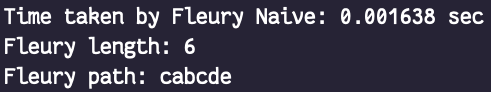
\includegraphics[width=1\linewidth]{Figuras/Fleury_naive.png}
  \captionof{figure}{Tempo de execução Fleury - Naive}
  \label{fig:naive}
\end{minipage}%
\hfill
\vline 
\hfill
\begin{minipage}{.48\textwidth}
  \centering
    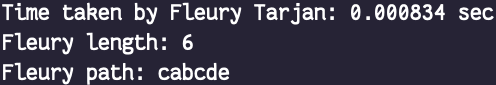
\includegraphics[width=1\linewidth]{Figuras/Fleury_tarjan.png}
  \captionof{figure}{Tempo de execução Fleury - Tarjan}
  \label{fig:tarjan}
\end{minipage}
\end{figure}

\newpage
\nocite{tarjan1974note}
\nocite{SCC}
\nocite{west_introduction_2000}